\section{Experiments}
\label{sec:experiments}

\begin{figure}[t]
\centering
	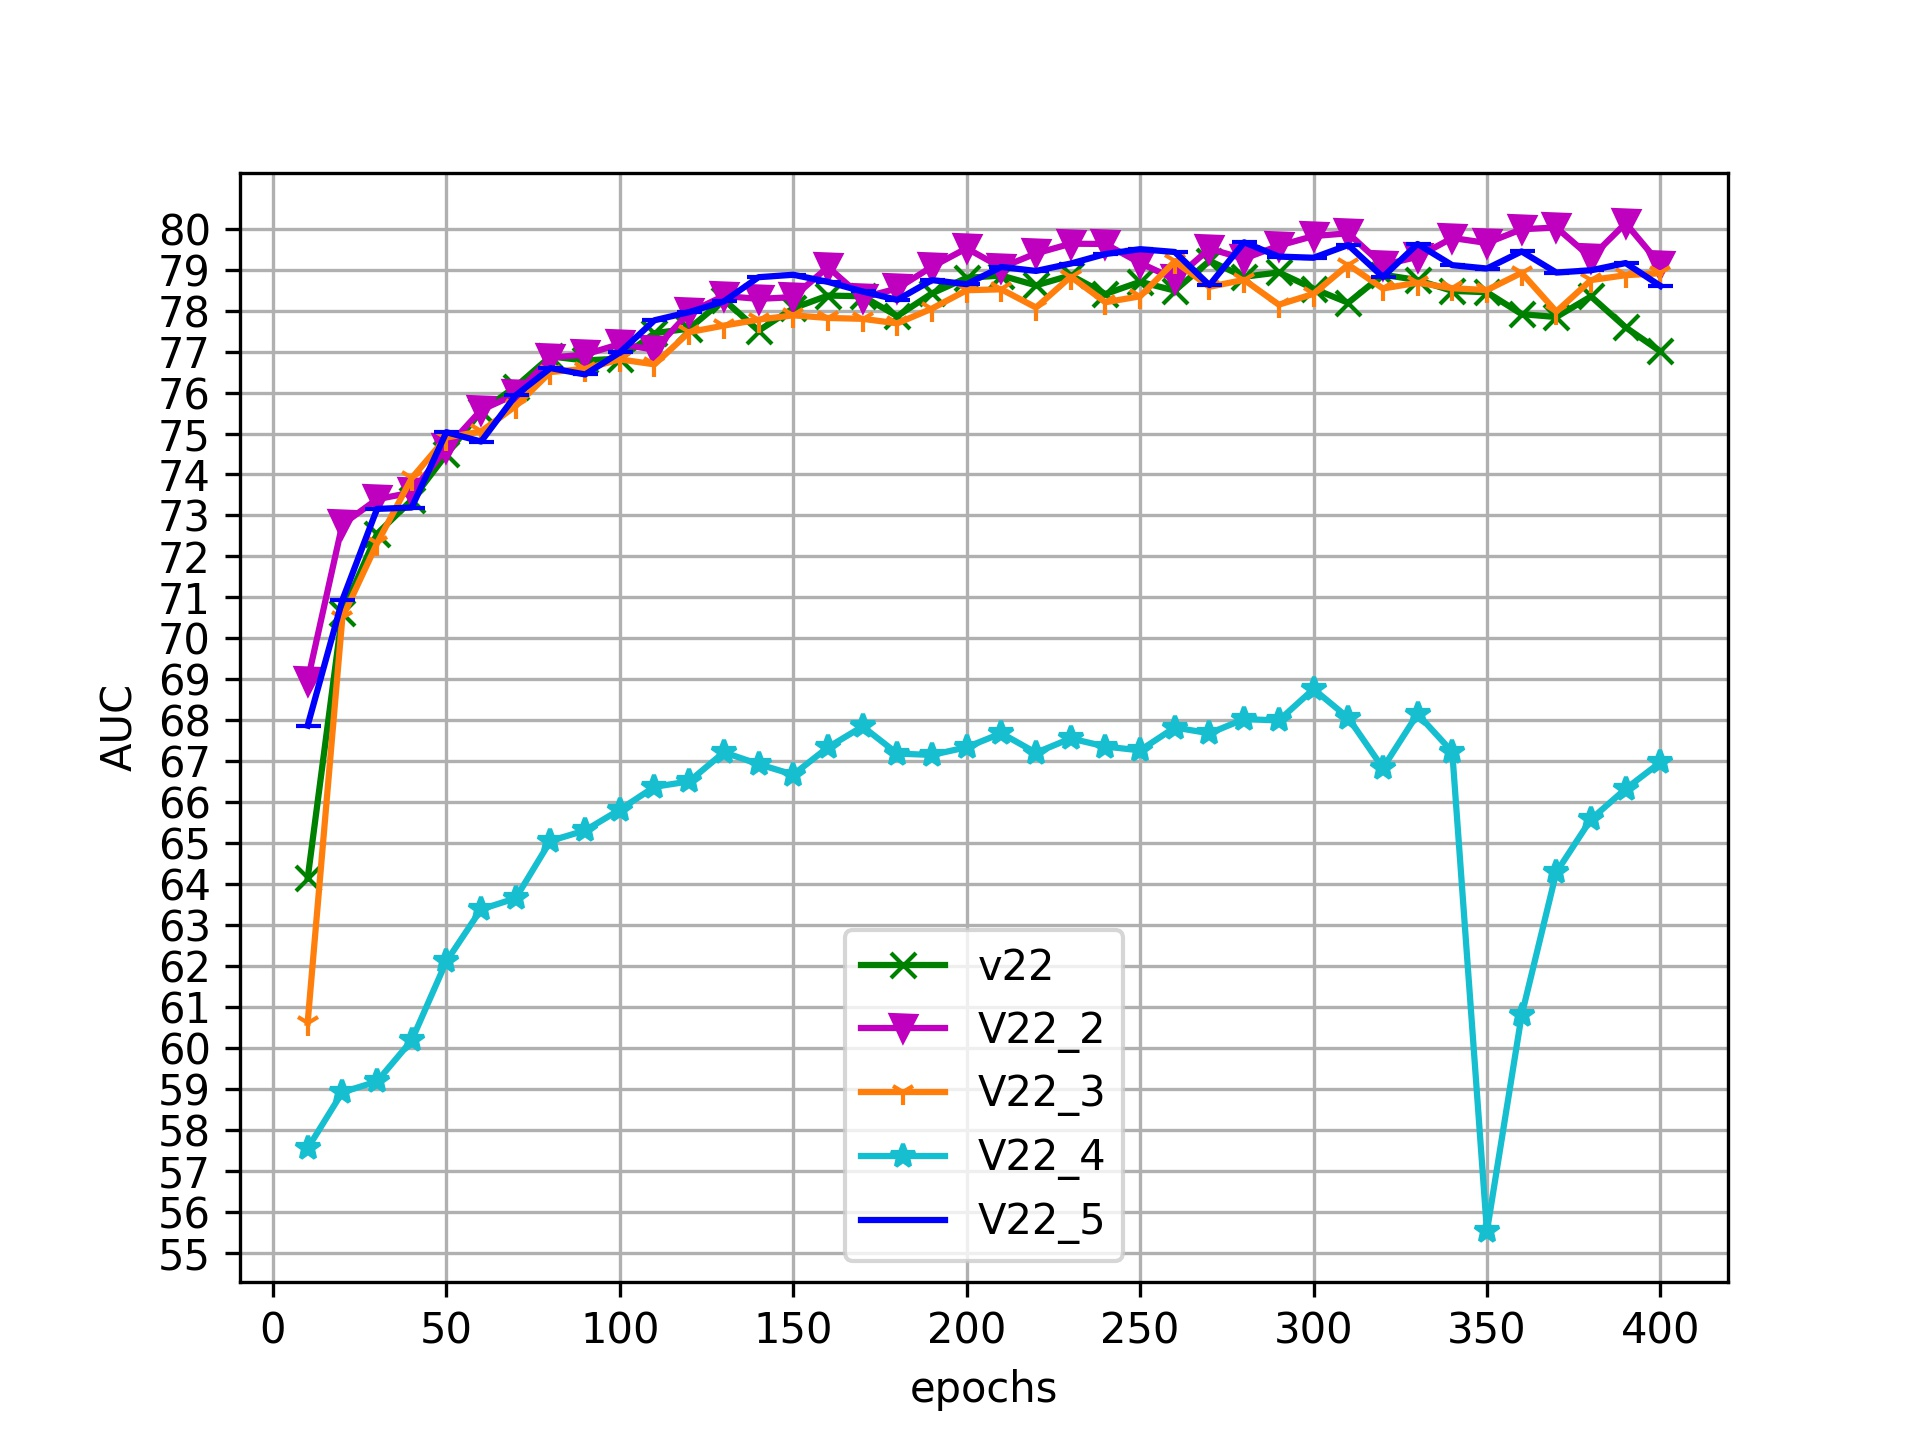
\includegraphics[trim=0 0 0 0, clip, width=1.\linewidth]{images/exp_1.jpg}
	\caption{Performance comparison changing the number of frames (from 1 to 5) in input of the Short-term memory module. NF: number of frames.}
	\label{fig:num-frames-vst}
\end{figure}

\begin{figure}[t]
\centering
	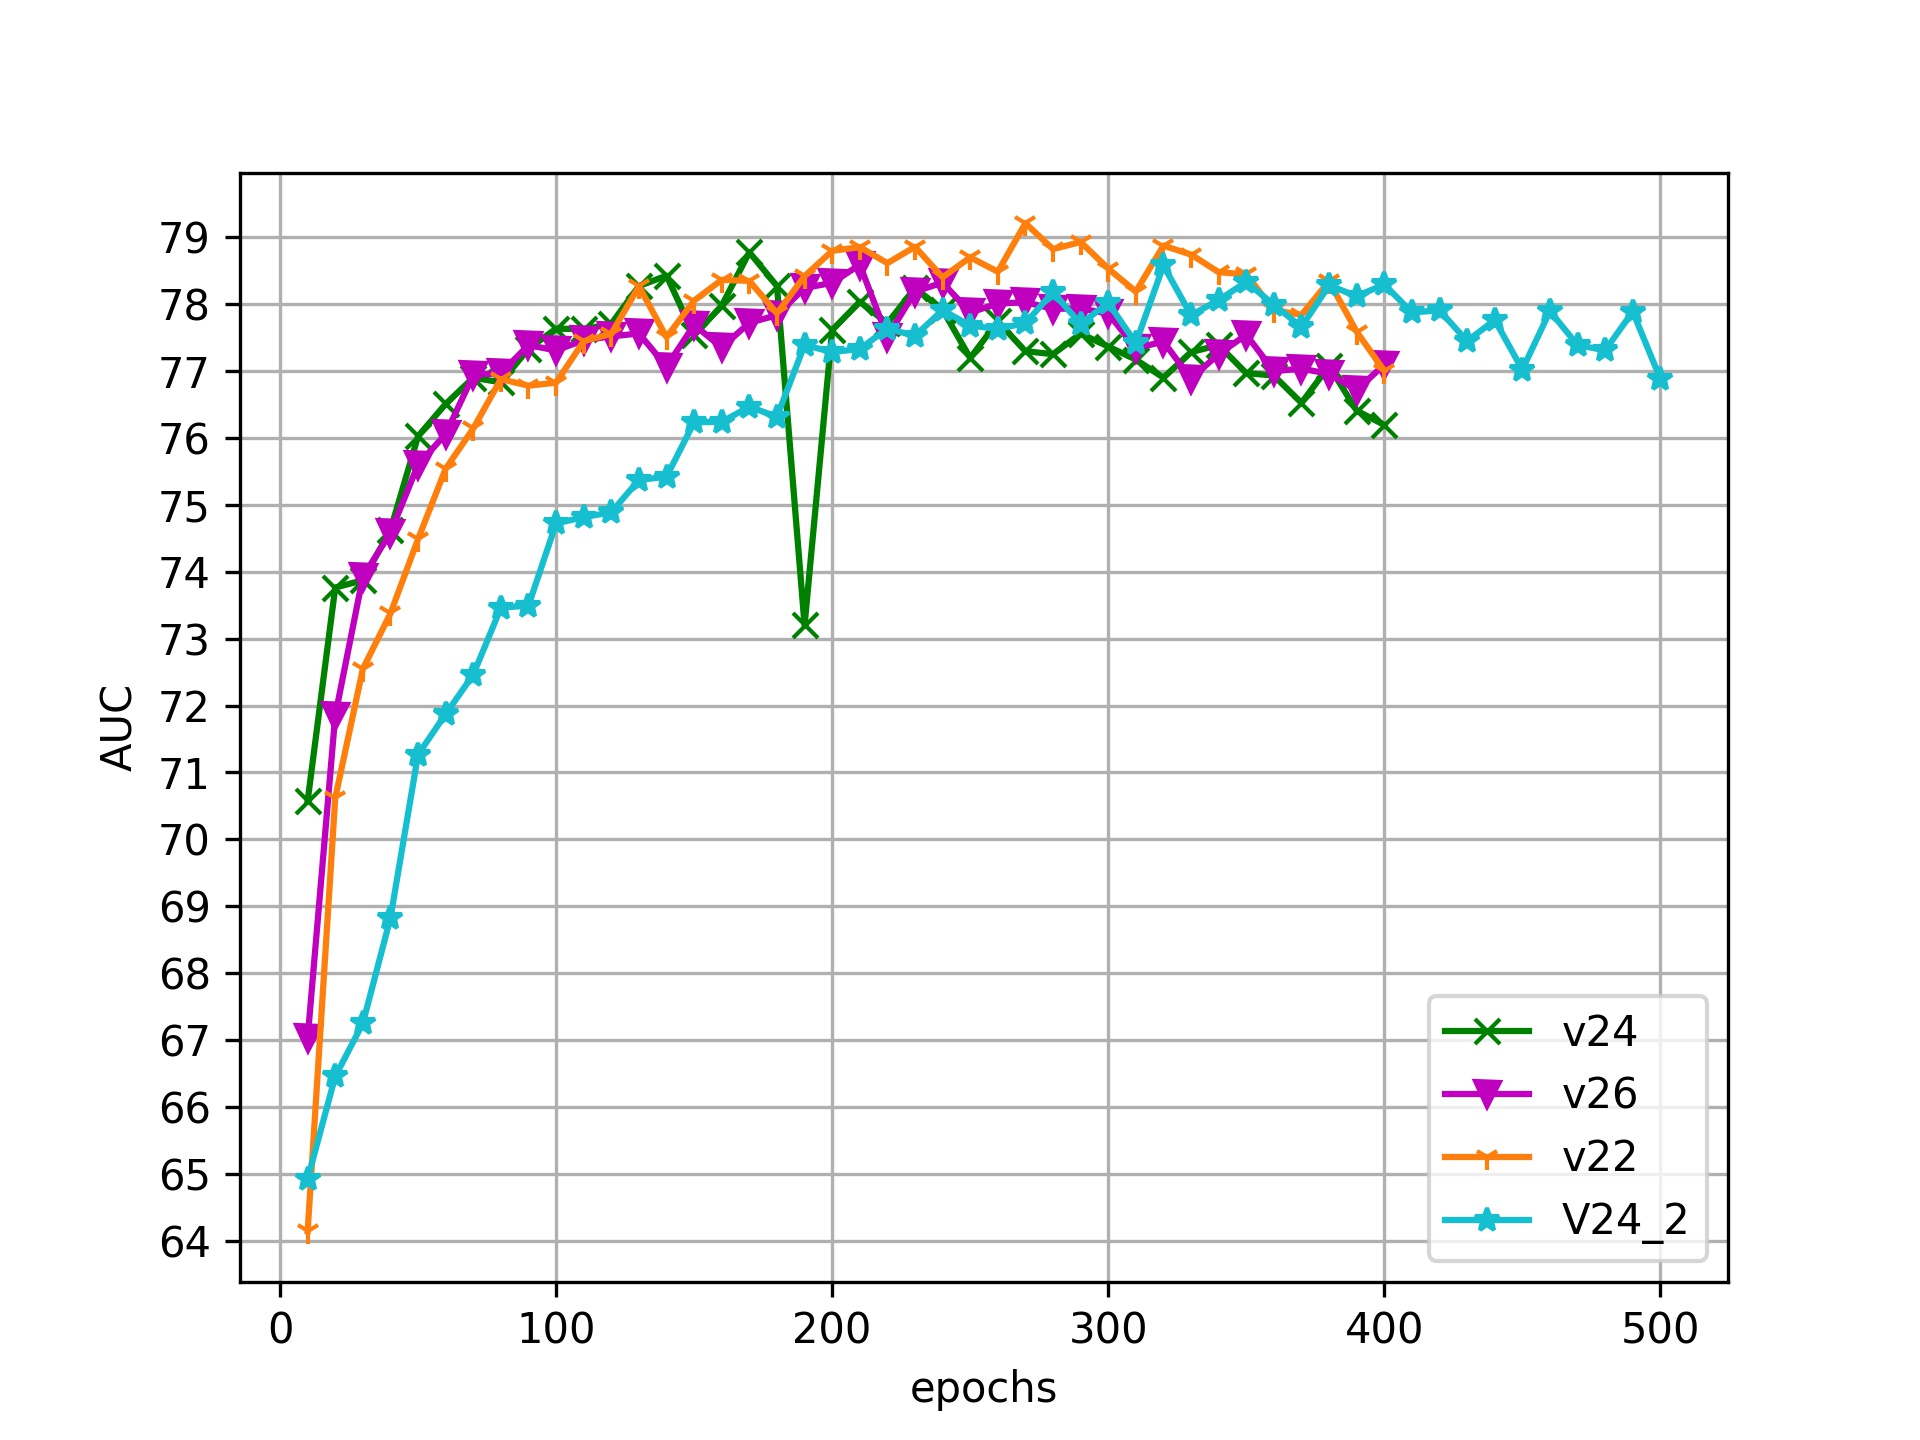
\includegraphics[trim=0 0 0 0, clip, width=1.\linewidth]{images/exp_2.jpg}
	\caption{Performance comparison changing the number and type of (long-term) memory cells (from 1 to 4).}
	\label{fig:num-memory-cells}
\end{figure}

\begin{table}[b]
	\footnotesize
	%\setlength{\tabcolsep}{1.2pt}
	\begin{center}
		\begin{tabular}{!c|^l|^c|^c|}
			\# & Type & \# cells & $AUC$ \\
			\hline\hline
			        % ??
			          1 &      &   & \\
			        % v24
			          2 & LSTM & 1 & \\
                    % v26
			          3 & GRU  & 1 & \\
			        % v22
		       	    4 & LSTM & 2 & 79.21 \\
	    	        % v26_2
		       	    5 & GRU  & 2 &  \\
	       	          % v24_2
                    6 & LSTM & 3 & \\
		              % v26_3
                    7 & GRU  & 3 & \\
                    % v24_3
                    8 & LSTM & 4 & \\
                    % v27_2
                    % 8 & LSTM &
	\end{tabular}
	\end{center}
	\caption{Study of long-term memory effect. Type: memory cell type. If not defined means no memory cell (neither following Linear) is inside the model. Row \#4 is $NF 3$ of previous experiment in Figure \ref{fig:num-frames-vst}.}
	\label{tab:long-term-memory-effect}
\end{table}

% TODO check se lasciare solo la figura o aggiungere anche la tabella!
\begin{table}[b]
	\footnotesize
	%\setlength{\tabcolsep}{1.2pt}
	\begin{center}
		\begin{tabular}{!c|^r|^c|}
			\# & \# Frames &  $AUC$ \\
			\hline\hline
			        % v28
			          1 & 4 & \\
			        % v22
			          2 & 8 & 79.21 \\
                    % v28_3
			          3 & 12 & \\
			        % v28_4
		       	    4 & 16 & \\
	    	        % v28_5
		       	    5 & 20 &  \\
	       	          % v28_6
                    6 & 24 & \\
\end{tabular}
	\end{center}
	\caption{Study the effect on training of the number of frames per video. Row \#2 is $NF 3$ of previous experiment in Figure \ref{fig:num-frames-vst}.}
	\label{tab:random-batch}
\end{table}

\noindent\textbf{Dataset}.
We perform our tests on the Dota dataset \cite{9712446}.
It contains 4677 videos taken from YouTube channels, with a resolution of $1024 \times 720$, annotated with information about the start and end of the anomaly, the category (10 in total) and the bounding boxes of the objects or persons involved.
The videos were recorded in different countries and with different light and weather conditions.
The dataset is split in approximately $70\%$ training and $30\%$ validation.
\lnote{li vogliamo ignorare o no?}
Because our benchmarks are related to the Task 1 \cite{9712446}, (online) frame-level Video Anomaly Detection, we ignore videos with unknown category or without objects, resulting in 1,305 test videos.
Furthermore, VO and OO columns are not shown because they do not contain anomalous traffic participants.

\noindent\textbf{Evaluation Metrics}.
To evaluate the performance of the models, we use the well-known Area Under Curve (AUC) metric.
This metric evaluate how well the model temporary-locate the anomaly in the videos.

\noindent\textbf{Implementation details.}
The results of the models with which we compare our model, are taken from the respective papers.
We perform the training on a single machine with 1 A100 GPU.
We use the Stochastic Gradient Descent (SGD) optimization algorithm with a learning rate of 0.0001 and a momentum of 0.9.
We decided to use SGD instead of Adam because in our experiments the latter led the training too much unstable, leading the model to diverge after a few epochs.

\noindent\textbf{Training details.}
Because the videos contain a non-uniform number of frames, to be able to fast training with batch-size major then one, we fixed the number of frames for each video taken into account.
In each iteration we chose the starting frame for each video, adjusting the ground-truth accordingly, in a way to offer to the network as diverse as possible training and reduce the effect of overfitting.
Unless otherwise specified, the model is initialized using a uniform distribution for Linear weights, with a (semi) orthogonal matrix for LSTM modules and zero for bias parameters.
For the VST Network, the weights were initialized with a model pretrained on Something-Something v2.

\subsection{Ablation study}

% class weight loss
% 2xsoftmax vs 1x
% learning rate differences (sto finendo l’esperimento con multipli lr)

\noindent\textbf{Short-term memory module.}

% v22: numero di frames in input
In this experiment, we empirically show the effect of the input frames to the Short-term memory module, varying the number of frames processed by the VST at each step.
The results are displayed in the Figure \ref{fig:num-frames-vst}.
As we expected, taking into account only the current frame is the worst situation, because an anomaly can only be recognized by processing a wider time frame.
With 4 frames we have the best result.
Increasing the number of frames processed at each step has a much more limited effect.
While, already with 5 frames the effect become counterproductive.

% v23: rand frame order (v17) vs normal
% training from scratch vs pretrained (imagenet vs smth2smthv2)

\noindent\textbf{Long-term memory module.}
% posizione dell'lstm senza / prima / dopo / prim + dopo / gru
% v2X: senza lstm
% v24, v22, v24_2: 1/2/3 # celle lstm
% v26, v26_2, v26_3: 1/2/3 # celle gru
% v27, v27_2: pre + post lstm (1 cell) + saliency (?), pre + post lstm (1 cell)
In this experiment, we evaluate the long-term memory effect on the classification capability.
In Figure \ref{fig:num-memory-cells}, we compare the network with and without the long-term memory.
For the long-term memory we test the LSTM and the GRU modules, with a number of cells varying from 1 to 3.

\noindent\textbf{Saliency module.}
% v25, v22: con/senza/versione ridotta della saliency
In this experiment, we evaluate the effect of the saliency branch.

\noindent\textbf{Video clip length.}
% v22, v28: random_batch 4/8/12/16/20/24: describi la modalità di addestramento -> per usare un batch size > 1 si è scelto di selezionare un numero max di frame da elaborare a ogni iterazione. per aggiungere diversità al training, il punto di inizio per ogni video viene scelto in modo casuale a ogni iterazione, adattando di conseguenza il ground-truth
As mentioned at the beginning of the section, at each iteration, a random starting point of the video is selected and a fixed number of video frames is used to train the network.
In Table \ref{tab:random-batch}, we evaluate the effect of the size of the video sub-sample on training.

\noindent\textbf{XXXX model}
% input shape
% versione finale vs resto del mondo su dota, and: 
%   - Phantom: https://paperswithcode.com/paper/approaches-toward-physical-and-general-video
%   - ShanghaiTech: https://paperswithcode.com/sota/anomaly-detection-on-shanghaitech
%   - CUHK Avenue: https://paperswithcode.com/sota/anomaly-detection-on-chuk-avenue
%   - UCSD Ped2: https://paperswithcode.com/sota/abnormal-event-detection-in-video-on-ucsd
Finally, we compare our architecture performance with state of the art models.